\section{Sequence Tagging Tasks}
\label{sec:SeqTagging}
We evaluate different word representations in four different sequence tagging tasks: POS-tagging, chunking, NER and MWE identification. 

For each sequence tagging task, we fed features into a first order linear-chain graph
transformer~\cite{collobert2011natural}, which contains two layers, as illustrated in Figure \ref{fig:graph_transformer}. The upper layer is identical to a linear-chain CRF~\cite{lafferty2001conditional}, the lower layer consists of word representation and hand-crafted features. If we treat word representations as fixed, the graph transformer is a linear-chain CRF. Alternatively, we can treat the word representations as model parameters, in which case the model is a neural network with word embeddings as the input layer. We trained all models with the online learning algorithm AdaGrad~\cite{duchi2011adaptive}. 

\begin{figure}[hb]
  \centering
  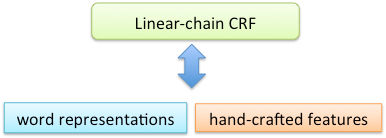
\includegraphics[scale = 0.3]{images/graph_transformer.png}
  \caption{Architecture of linear-chain graph transformer}
  \label{fig:graph_transformer}
\end{figure}


As in~\cite{turian2010word}, at each word position, we extract word representation features from the words in a window $\{-2, -1, 0, 1, 2\}$. The word representation features of word embeddings are the pre-trained continuous vectors of each word.  The Brown clustering features are the prefix features extracted from word clusters in the same way as~\cite{turian2010word}. In addition, we include one-hot representation of unigrams for comparison as well.

For POS-tagging, chunking and MWE, we used the same hand-crafted features as the state-of-the-art approaches,  \newcite{collobert2011natural}, \newcite{turian2010word} and ~\newcite{mwecorpus}, respectively. For NER, we considered the same feature space as in~\cite{turian2010word}, except for the previous two predictions, because we want to evaluate all word representations with the same type of model -- first-order graph transformer.

During training of distributed representation of words, we consider two settings: 

\begin{small}
\begin{itemize}
\item[-] Graph transformer \textit{does not} fine tune word representations during training. 
\item[-] Graph transformer fine tunes the word representations during training. 
\end{itemize}
\end{small}

\begin{table*}
\caption{Datasets splits and feature space for each sequence tagging task.}
\begin{small}
\begin{tabular}{lllp{3.cm}ll}
\hline
			& \textbf{Training set} & \textbf{Validation set} & \textbf{\textit{in-domain} Test set} & \textbf{\textit{out-of-domain} Test set} \\ \hline
\textbf{POS-Tagging} & 0-18 WSJ & 19-21 WSJ & 22-24 of WSJ & English Web-Treebank  \\
\textbf{Chunking} & WSJ & 1000 sentences WSJ & CoNLL-2000 & Brown corpus \\
\textbf{NER} & CoNLL-2003 train set & CoNLL-2003 dev. set & CoNLL-2003 test set & MUC7  \\
\textbf{MWE} & 500 documents from & 100 documents from & 123 documents & - \\
\hline
\end{tabular}
\label{datasplit}
\end{small}
\end{table*}

We split the task specific corpus into a training set, validation set, and a test set (see Table \ref{datasplit}). If a corpus already provides fixed splits, we reuse them. For POS-tagging,  NER and chunking, we also evaluated the models with a out-of-domain corpus (English Web-Treebank, MUC-7 and Brown corpus, respectively), which has similar annotation schema as the respective training corpus.

In order to have fair and reproducible experimental results, we tuned the hyperparameters with random search~\cite{bergstra2012random}. 
We randomly sampled 50 distinct hyperparameter sets with the same random seed for the models that do not update word embeddings, and sampled 100 distinct hyperparameter sets for the models that update word embeddings. 
For each set of hyperparameters, we train a model on its training set and pick up the best one based on its performance on its validation set~\cite{turian2010word}. 
Note that, we also consider word vector size and context window size of distributed word representation, and number of clusters of brown clustering as the hyperparameters.
This is achieved by mapping each possible hyperparameter combination to the word representation files trained with these parameters. 

However, for the models that update word representations, we always found under-performed hyperparameters after trying out all hyperparameter combinations, because they have more hyperparameters than the models that do not update word representations. Then, for each distributed word representations, we reuse all hyperparameters of the models that do not update word representations, only tune the hyperparameters of AdaGrad for the word representation layer. This method requires only 32 additional runs for each model updating embeddings and achieves consistently better results than 100 random draws.

The final evaluation is carried out in a semi-supervised setting. We split the training set into 10 partitions at log scale. That means, the second smallest partition will be twice the size of the smallest partition. We created 10 training sets with incremental size by merging these partitions from the smallest one to the largest one, and each of them on the same designated test sets. 

For easy comparison with previous results, we adopted the most widely used F1 measure as the evaluation metric for all tasks except POS-tagging, for which we use per-word accuracy. In order to evaluate model performance on out-of-vocabulary (unknown) words, we reported also the accuracy for the words that do not occur in the training set.

%\subsection{POS-tagging} We could choose one of the options. \subsubsection{Option 1} Almost the same setting as~\cite{collobert2011natural}, except adding one more test set.
% \noindent Training set: 0-18 of WSJ.
% \noindent Validation set: 19-21 of WSJ.
% \noindent Test set: 22-24 of WSJ, and English Web Treebank. We report model performances on these two test sets respectively.
% \noindent Feature space: the same set as in~\cite{collobert2011natural}

% \subsection{Chunking} The same setting as~\cite{turian2010word}\\
% \noindent Training set: WSJ train set.
% \noindent Validation set: Randomly sampled 1000 sentences from the train set for development.
% \noindent Test set: CoNLL2000 test set.
% \noindent Feature space: the same set as in~\cite{turian2010word}

% \subsection{MWE Identification} Training set: randomly sampled 500 documents from Nathana��s corpus. 
% \noindent Validation set: randomly sampled 100 documents from Nathana��s corpus.
% \noindent Test set: remaining 123 documents from Nathana��s corpus..
% \noindent Feature space: the same set as in~\cite{mwecorpus}

%\subsection{Named entity recognition} Training set: CoNLL03 train set.
% \noindent Validation set: CoNLL03 development set.
% \noindent Test set: CoNLL03 test set and MUC7. We report model performances on these two test sets respectively.
% \noindent Feature space: the same set as in~\cite{turian2010word}